\section{Tasks}
\label{sec:tasks}

The Scenario Checker has two modes: Recording and Playback. 
The mode of the Scenario Checker is shown in the label at the top of the control panel (see Fig. \ref{fig:changingMode}).

\begin{figure}[!htbp]
	\centering
	\ifplastex
	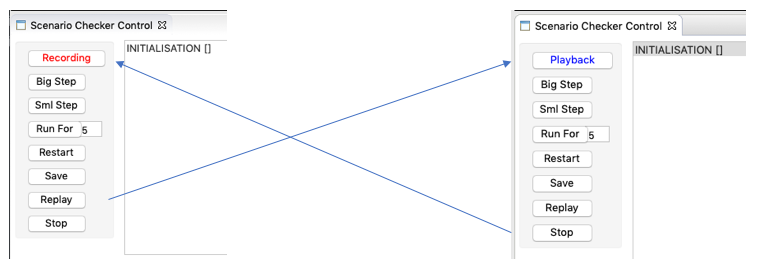
\includegraphics[width=768]{figures/changingMode}
	\else
	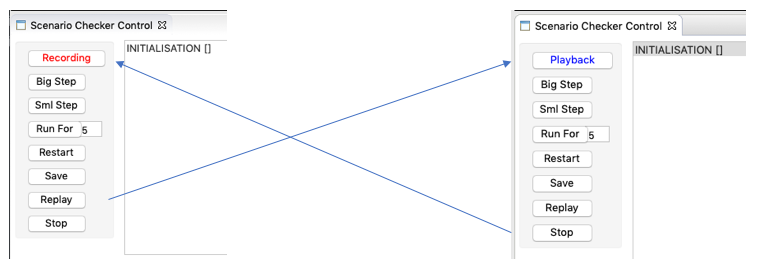
\includegraphics[width=0.9\textwidth]{figures/changingMode}
	\fi
	\caption{Changing Mode in the Scenario Checker}
	\label{fig:changingMode}
\end{figure}


The Scenario Checker is always started in the recording mode.
It changes to playback mode when the mode indicator button is pressed while it displays recording.
It changes to recording mode when the mode indicator button is pressed while it displays playback.

\subsection{Recording a Scenario}
\label{sec:recording}

With the Scenario Checker in recording mode, the user can choose from the available external events and arguments that are listed in the Scenario Checker Control Panel (see lower left view in Fig. \ref{fig:recording}). 
The chosen  event is executed (either by double clicking on it, or selecting it and then pressing the Big Step button).
The Scenario Checker automatically runs internal events until completion and then updates the Scenario Checker State view to show the state of all non-private variables.

At any point, after firing a sequence of events, the scenario can be saved without altering the current scenario execution. 
This makes it easy to record intermediate points in a scenario.
The ProB history view can be used to return to any point in the scenario history.
For example if the user makes a mistake or decides that a different event trace would have been better, the ProB History view can be used to discard the later part of the trace and a new sequence can be continued from that point on.
(Note that, when saving, the scenario execution is always obtained from the ProB animation history, rather than any user interaction with the Scenario Checker).

In recording mode, the Scenario Checker Control Panel buttons have the following function:
\begin{itemize}
	\item \textbf{Mode (Recording)}  Switches to playback mode and allows the user to select a previously recorded scenario oracle file to play. This discards the current scenario after a warning confirmation from the user.
	\item \textbf{Restart}  Discards the current scenario and restarts animation from the \texttt{INITIALISATION}. If the scenario had progressed beyond the \texttt{INITIALISATION} event, a warning and confirmation message box is displayed.
	\item \textbf{Save}  Saves the current scenario and continues without interruption. This enables common prefixes to be saved as partial scenarios for later completion. The scenario is saved in a folder called \texttt{Oracle} inside the Event-B project. The filename is automatically constructed from the machine name and a timestamp with the extension, \texttt{.oracle}.
	\item \textbf{Big Step}  Executes events until completion of the next big step. If an operation has been selected from the list of enabled external events in the Scenario Checker Control Panel (by single clicking on it), that event will be executed. If no such event is selected, one will be picked at random. In either case, if after executing the external event any internal events are enabled, one will be executed at random and according to any priority that has been defined in the model (see Section \ref{sec:concepts}). Firing of internal events will continue in this way until none are enabled or a loop is detected. (A loop is detected when the same event has already been executed in this run to completion). Double clicking on an event in the list of enabled events in the Scenario Checker Control Panel is exactly the same as selecting the event and using the big step button.
	\item \textbf{Small Step}  Executes one event which is selected as follows. If an operation has been selected from the list of enabled external events in the Scenario Checker Control Panel (by single clicking on it), that event will be executed. Otherwise, if any internal events are enabled, one will be executed at random and according to any priority that has been defined in the model (see section \ref{sec:concepts}). Note that it is possible to ignore internal events using the small step button which may lead to scenarios that fail when played back (since it is not usual behaviour to ignore internal events).
	\item \textbf{Run For..}  Executes the number of big steps shown in the text box next to the button. The number can be changed by clicking in the box and editing the number.
\end{itemize}

In recording mode, if the scenario has progressed beyond \texttt{INITIALISATION} (i.e. there is a useful scenario that could be saved) the Scenario Checker Control Panel indicates that a scenario could be saved by displaying an \texttt{*} in the title bar.

In recording mode the Scenario Checker View displays the current value of all non-private variables irrespective of whether they have changed or not.
The Expected value column is left blank.

\begin{figure}[!htbp]
	\centering
	\ifplastex
	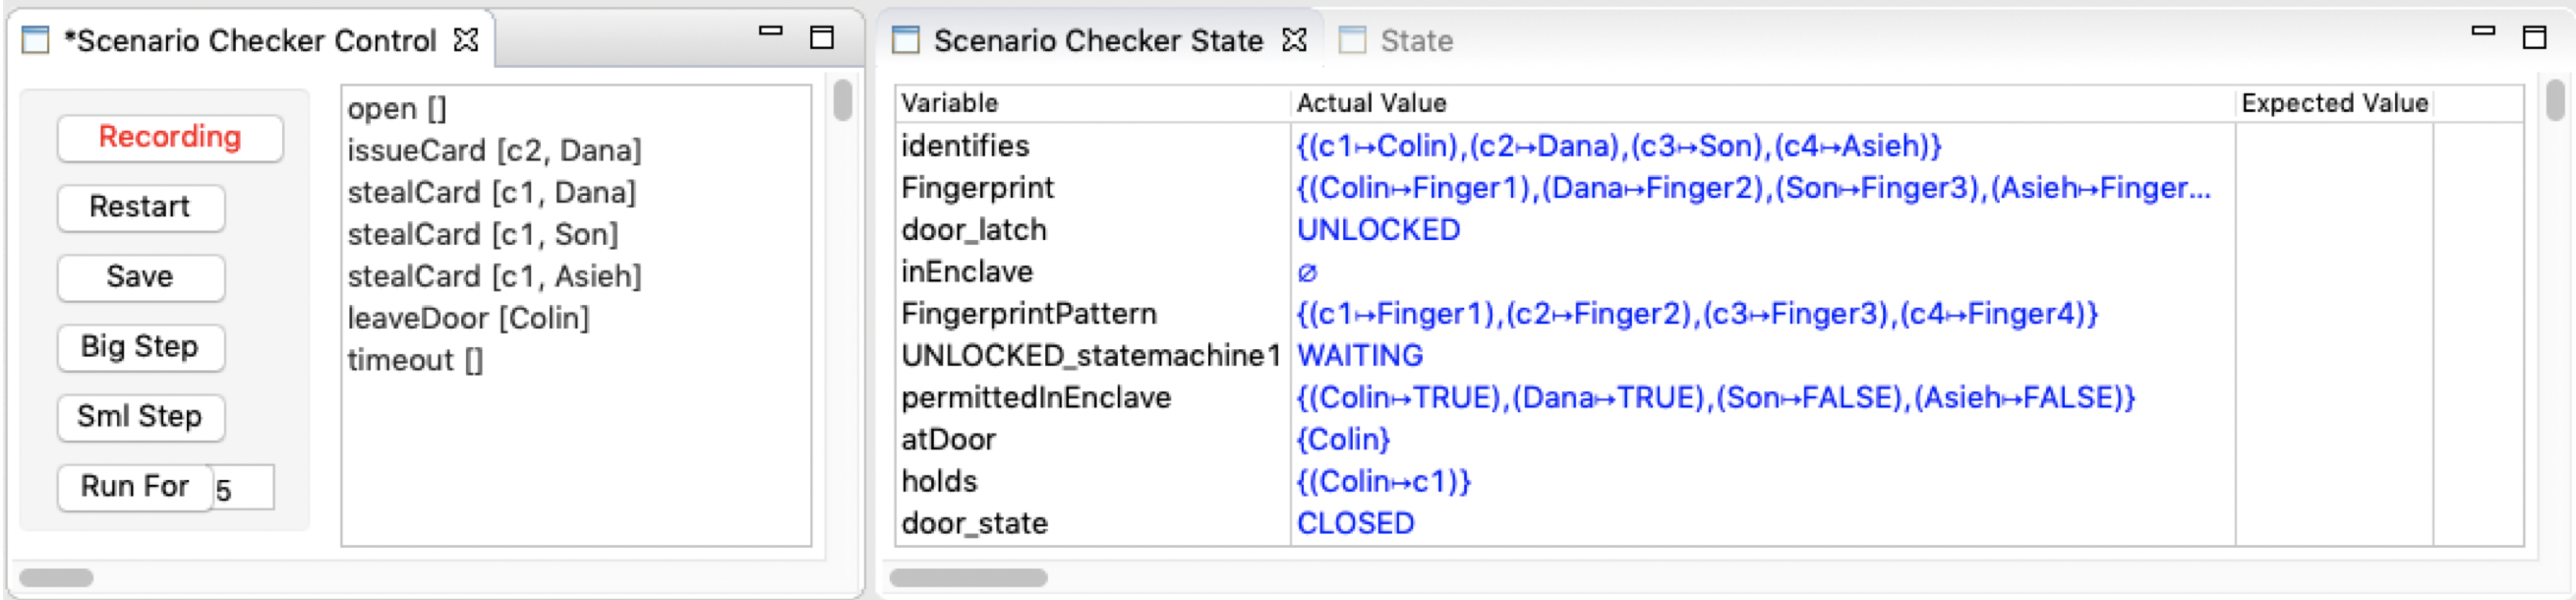
\includegraphics[width=900]{figures/recording}
	\else
	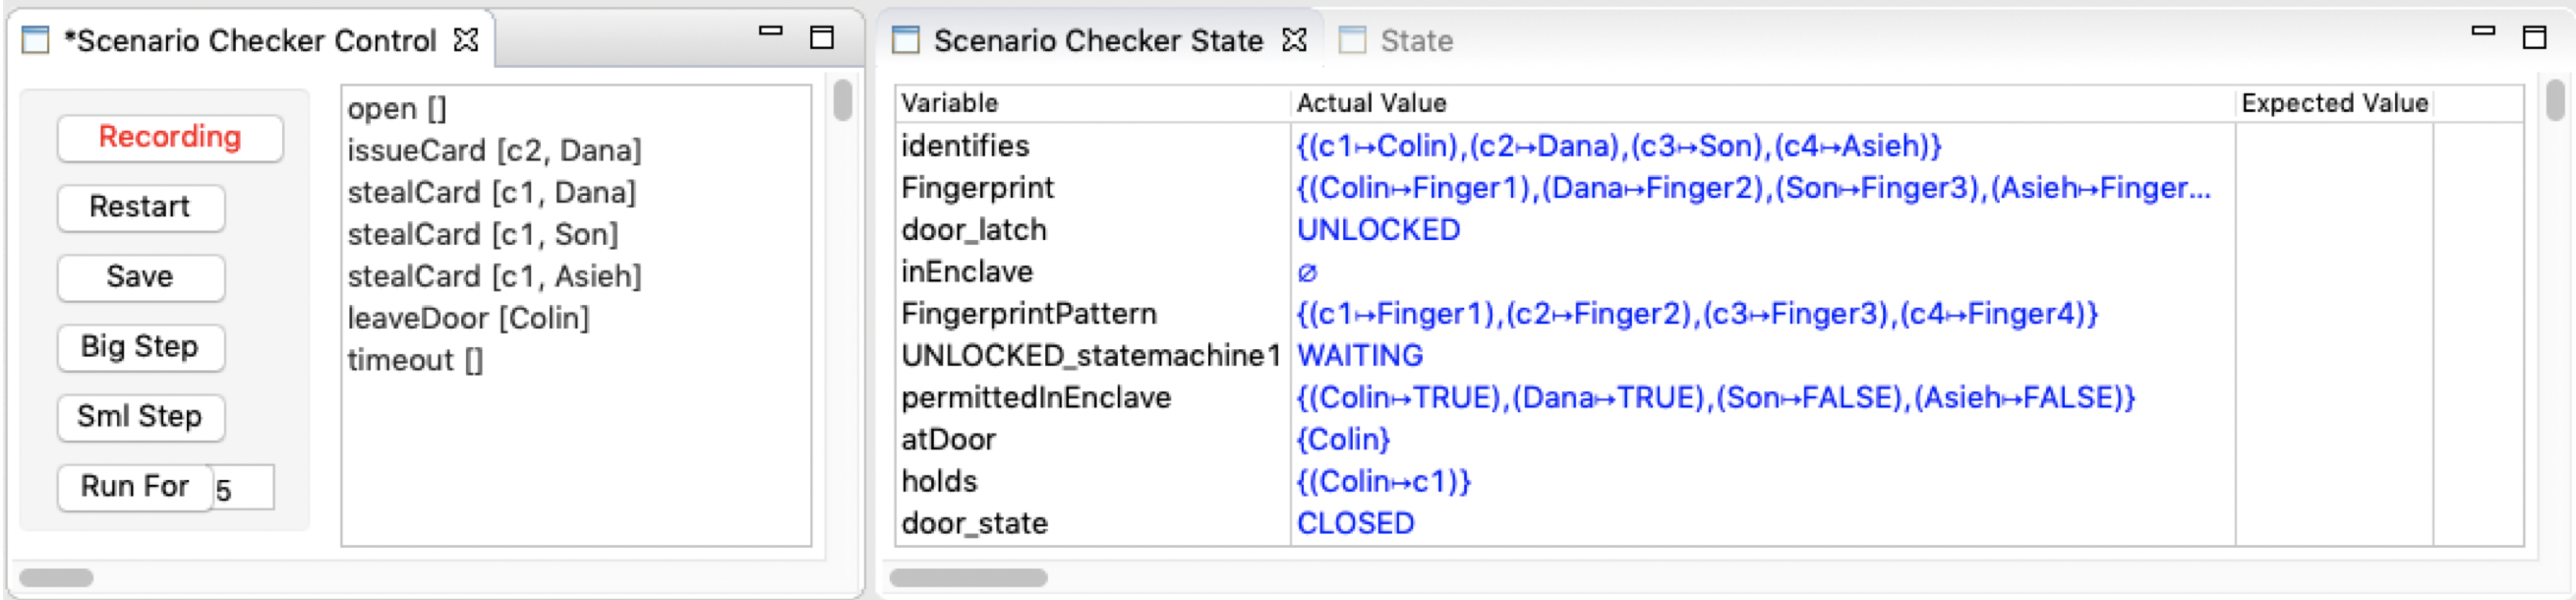
\includegraphics[width=0.9\textwidth]{figures/recording}
	\fi
	\caption{Scenario Checker in Recording Mode}
	\label{fig:recording}
\end{figure}

\subsection{Re-playing a Scenario}
\label{sec:playback}

With the Scenario Checker in playback mode (see Replay button in Section \ref{fig:recording}), the execution of events is taken from the scenario oracle file being replayed.
The user should not try to control the execution of events and an information message will be displayed if she attempts to select events from the Scenario Checker Control Panel. 
(Note that it is not possible to prevent other animation plug-ins (including the ProB `Events' view) from executing events but this would most likely make the scenario fail. 
The user presses the Big Step button to tell the Scenario Checker to execute the next recorded external event followed by any enabled internal events (similar to in recording mode).
The Scenario Checker then updates the Scenario Checker State view to show the state of any non-private variables that have changed state.
The expected value from the recording is shown and any differences are highlighted in red.
At any point, the playback can be stopped and an alternative ending can be recorded.

In playback mode, the Scenario Checker Control Panel buttons have the following function:
\begin{itemize}
	\item \textbf{Mode (Playback)}  Switches to recording mode. The scenario execution is left in whatever state it was during the playback. This allows multiple alternative scenarios to be recorded using a common recorded prefix.
	\item \textbf{Restart}  Discards the current scenario execution and restarts the same recorded scenario animation from the \texttt{INITIALISATION}. 
	\item \textbf{Save}  Saves the current scenario execution and continues without interruption still in playback. This enables common prefixes to be saved as partial scenarios for later completion. The scenario is saved in a folder called `Oracle' inside the Event-B project. The filename is automatically constructed from the machine name and a timestamp with the extension, `oracle'. 
	\item \textbf{Big Step}  Executes events until completion of the next big step. The external event is taken from the recording. If, after executing the external event, any internal events are enabled, one will be executed at random and according to any priority that has been defined in the model (see section \ref{sec:concepts}). Firing of internal events will continue in this way until none are enabled or a loop is detected. (A loop is detected when the same event has already been executed in this run to completion).
	\item \textbf{Small Step}   Executes one event which is selected as follows. If any internal events are enabled, one will be executed at random and according to any priority that has been defined in the model (see section \ref{sec:concepts}). Otherwise, attempts to play the next external event from the scenario being played, but does not automatically fire subsequent internal events. Note that after firing a single step without firing the internal events, the state will probably not match the expected state in the scenario.
	\item \textbf{Run For..}   Executes the number of big steps shown in the text box next to the button. The number can be changed by clicking in the box and editing the number.
\end{itemize}

In playback mode, the next external event in the recorded scenario (i.e. the event that will be executed when the big step button is next pressed) is highlighted in the list of enabled external events in the Scenario Checker Control Panel.

In playback mode the Scenario Checker View displays the current value of any non-private variables that have changed value since the last step.
The Expected value column displays the corresponding value from the recorded scenario for comparison.
If the values are the same the current value is displayed in green. 
If the values differ the current value is displayed in red.

When all steps in the recorded scenario have been played, the user is prompted to switch to recording mode. 
The Scenario Checker switches to recording mode without disturbing the current state of the scenario execution. 
This allows the scenario to be extended to make a new, longer, recorded scenario.

\begin{figure}[!htbp]
	\centering
	\ifplastex
	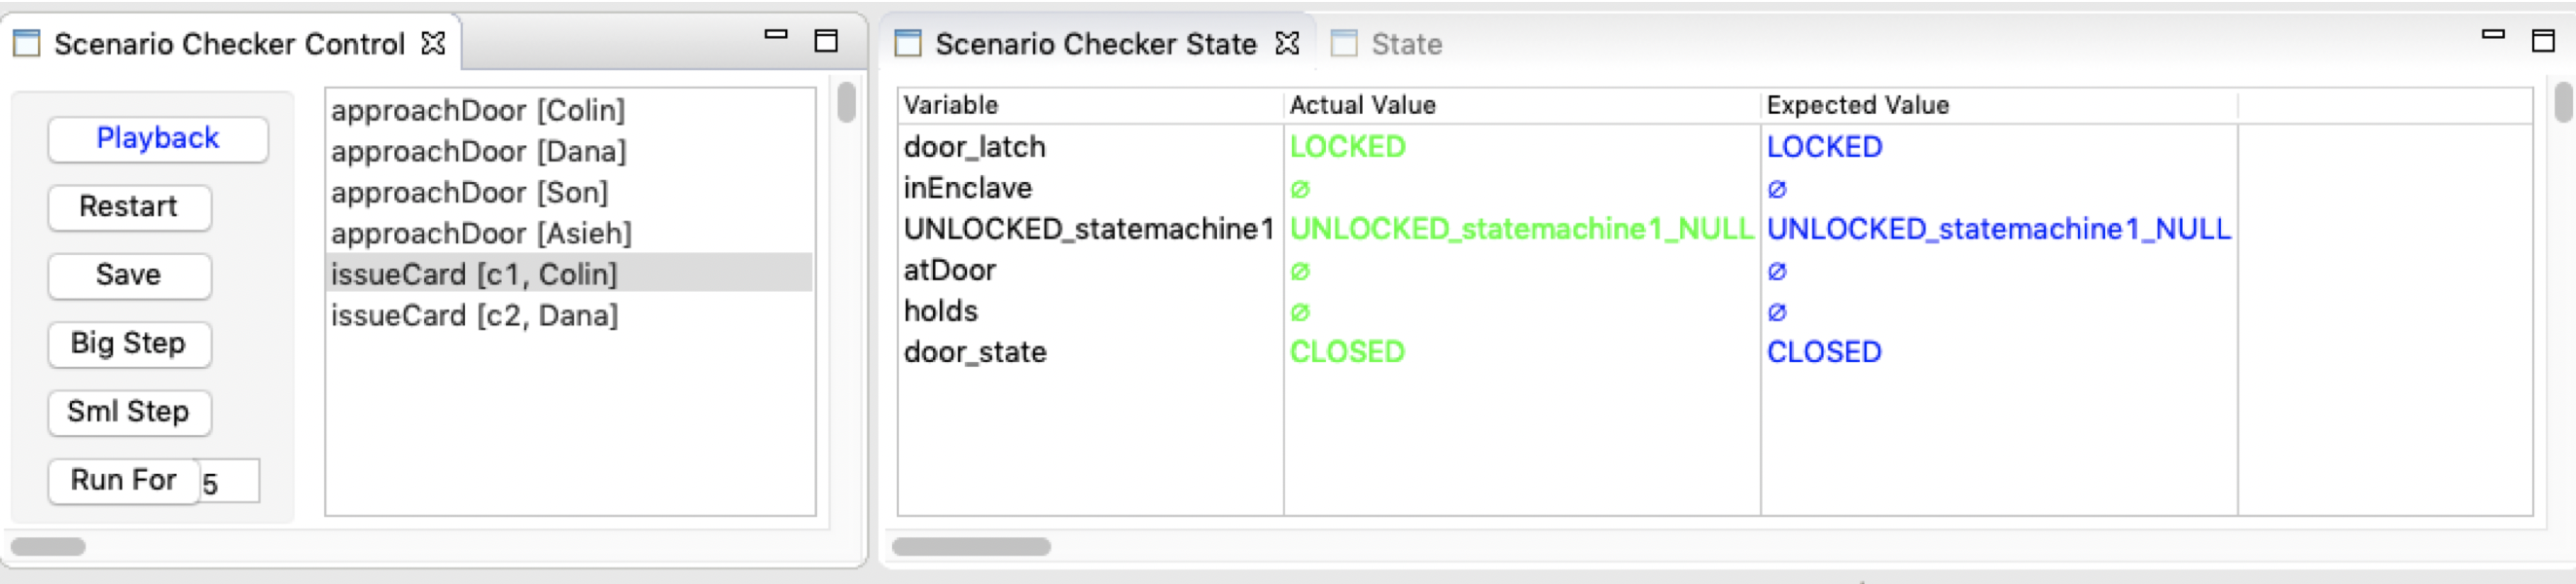
\includegraphics[width=900]{figures/playback}
	\else
	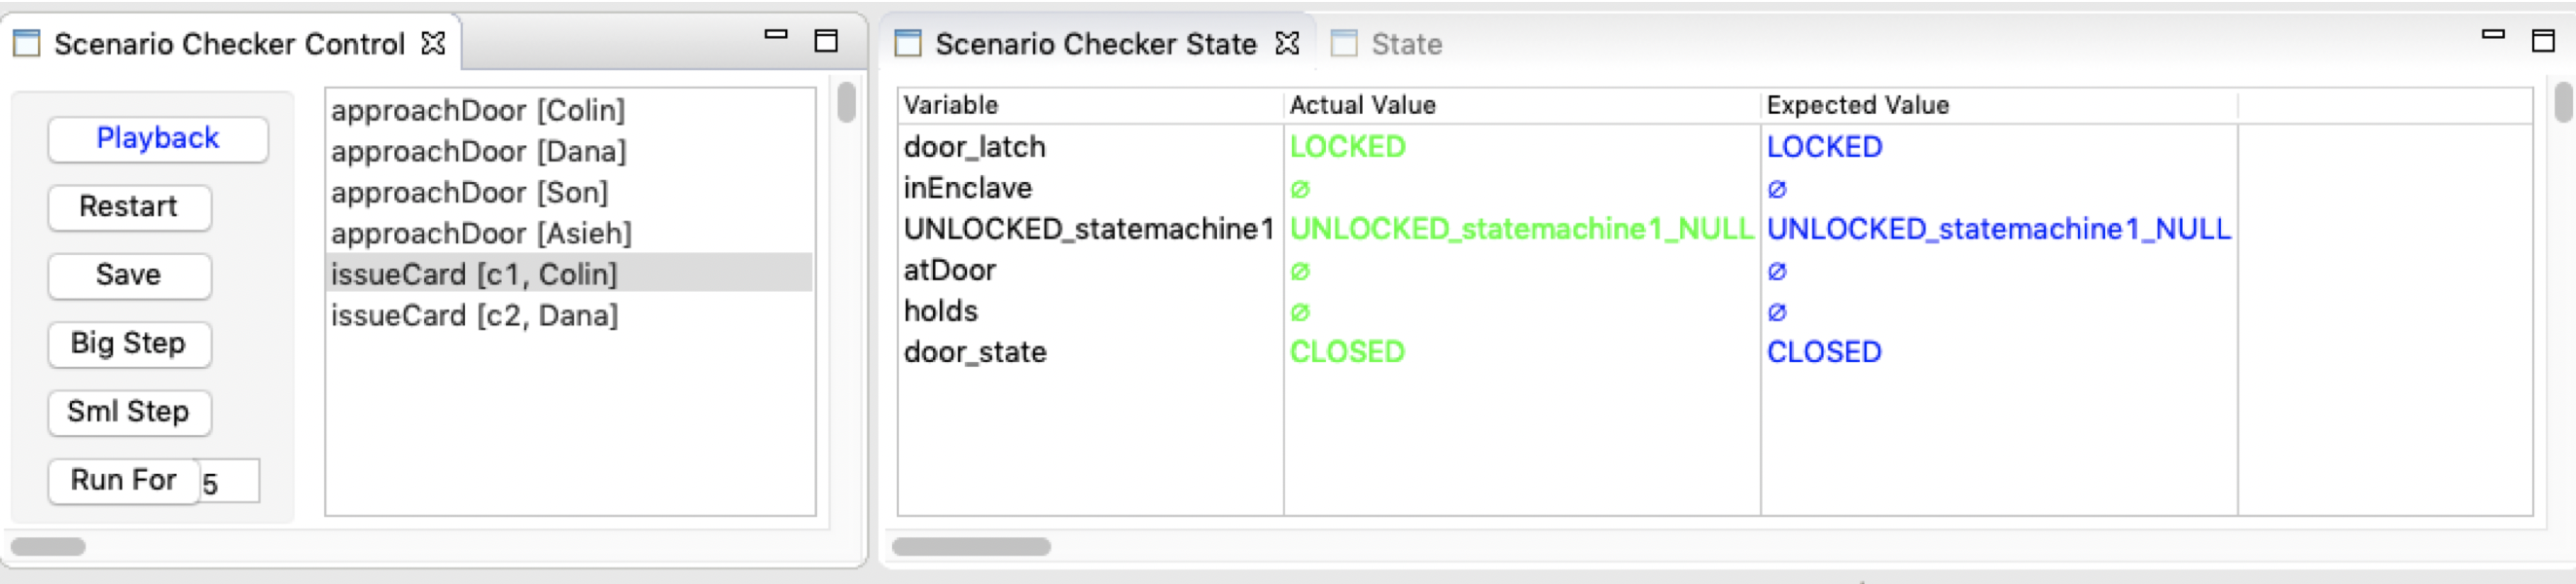
\includegraphics[width=0.9\textwidth]{figures/playback}
	\fi
	\caption{Scenario Checker in Playback Mode}
	\label{fig:playback}
\end{figure}
%%% Local Variables:
%%% mode: latex
%%% TeX-master: "user_manual"
%%% End:
